\qns{Resistance is not Futile!}

\textbf{Learning Goal:} Introduce the concept of resistivity and provide physical intuition for how changes in physical properties/dimensions of a resistor changes its resistivity. Read \notes{Note 12 Section 12.3-12.4} to learn more.

\meta{
\begin{itemize}
\item Having one consistent analogy throughout the question, such as a water pipe, can help give students a better mental image of what changes between parts.

\item Relate putting wires lengthwise to resistors in series and putting wires side to side to resistors in parallel.
\end{itemize}

}

Resistivity is a \textbf{physical property} of the material that quantifies how much it opposes the flow of electric current.

Assume that in an ideal case, the cross-section and physical composition of the wire are uniform, We can find its resistance with the equation below:

$$R = \rho \frac{L}{A}$$

Here, $\rho$ stands for the resistivity of the wire, $R$ stands for its resistance, $A$ stands for the area of the cross section of the wire, and $L$ stands for the length of the wire. 


We will be frequently referencing some of the following variables:
\begin{itemize}
    \item $A$: the cross section area of a single wire.
    \item $L$: the length of a single wire.
    \item $\rho_{cu}$: resistivity for the material copper.
    \item $\rho_{Al}$: resistivity for the material aluminum.
\end{itemize}


\begin{enumerate}
\item
A copper (Cu) structure with a square cross-section is shown below. Given the material parameters, calculate the resistance $R_{\mathrm{Cu}}$ of the structure between $E_1$ and $E_2$.

\begin{center}
\includegraphics[scale = 0.6]{../q_resistor_model_figs/fig1.png}
\end{center}

\begin{center}
\begin{tabular}{ |c|c| } 
 \hline
 $\rho_{\mathrm{Cu}}$ & $\SI{1e-8}{\ohm\meter}$ \\ 
 \hline
 $s_{\mathrm{Cu}}$ & $\SI{5}{\nano\meter}$ \\ 
 \hline
 $l$ & $\SI{75}{\nano\meter}$ \\ 
 \hline
\end{tabular}
\end{center}

\ans{

Using the formula for resistance $R$, we can find the resistance of the Cu structure given the resistivity and the dimensions:
\[R = \rho \frac{l}{A} \implies R_{\mathrm{Cu}} = \rho_{\mathrm{Cu}} \frac{l}{s_{\mathrm{Cu}}^2} = \SI{1e-8}{\ohm\meter} \cdot \frac{\SI{75e-9}{\meter}}{\left(\SI{5e-9}{\meter}\right)^2} = \SI{30}{\ohm}\]
}

\itemNow you are given a copper slab with dimensions $0.9\si{\centi\meter}$, $2.7\si{\centi\meter}$, and $7.7\si{\centi\meter}$ as denoted on the figure below. The dimensions and the resistivity of the slab remain the same throughout the rest of the problem. % $0.9 < 2.7 < 7.7$. 

\begin{figure}[h]
	\begin{center}
		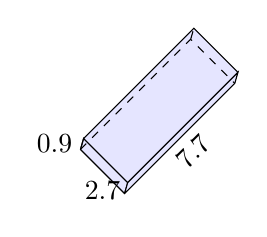
\begin{tikzpicture}[scale=1, x={(0.14cm,-0.14cm)},y={(0.04cm,0.14cm)},z={(-1.4cm,-1.4cm)}]
		\pgfmathsetmacro{\x}{4}
		\pgfmathsetmacro{\y}{1}
		\pgfmathsetmacro{\z}{1}
		\path (0,0,\y) coordinate (A) (\x,0,\y) coordinate (B) (\x,0,0) coordinate (C) (0,0,0)
		coordinate (D) (0,\z,\y) coordinate (E) (\x,\z,\y) coordinate (F) (\x,\z,0) coordinate (G)
		(0,\z,0) coordinate (H);
		\draw[fill=blue!10] (A)--(E)--(F)--(B);
		\draw[fill=blue!10] (A)-- node[below]{$2.7$} (B)-- node[below,sloped]{$7.7$} (C)--(G)--(F)--(B) (A)-- node[left]{$0.9$}(E)--(F)--(G)--(H)--(E);
		\draw [dashed,black] (A)--(D)--(C) (D)--(H);
		\end{tikzpicture}
	\end{center}
\end{figure}


Suppose we connect opposite faces of the slab to a voltage source so that current can flow through it. Notice that there are \textbf{3 possible configurations} we can have for this slab, leading to 3 possible directions in which the current can flow (drawn in the answer choices below). Which direction will lead to the \textbf{highest} current flow $I$ assuming we use the same voltage source all three times? 
\\
Assume the resistivity is the same throughout the slab and does not vary with respect to \newpage
\begin{multicols}{2}
  \begin{enumerate}
  	\setlength\itemsep{2cm}
\item Parallel to $0.9$ (current goes through $2.7$, $7.7$ face): \\
\begin{minipage}{0.5\linewidth}
    \begin{center}
        \begin{tikzpicture}[scale=2, x={(0.14cm,-0.14cm)},y={(0.04cm,0.14cm)},z={(-1.4cm,-1.4cm)}]
            \pgfmathsetmacro{\x}{4}
            \pgfmathsetmacro{\y}{1}
            \pgfmathsetmacro{\z}{1}
            \path (0,0,\y) coordinate (A) (\x,0,\y) coordinate (B) (\x,0,0) coordinate (C) (0,0,0)
            coordinate (D) (0,\z,\y) coordinate (E) (\x,\z,\y) coordinate (F) (\x,\z,0) coordinate (G)
            (0,\z,0) coordinate (H);
            \draw[fill=blue!10] (A)--(E)--(F)--(B);
            \draw[fill=blue!10] (A)-- node[below]{$2.7$} (B)-- node[below,sloped]{$7.7$} (C)--(G)--(F)--(B) (A)-- node[left]{$0.9$}(E)--(F)--(G)--(H)--(E);
            \draw [dashed,black] (A)--(D)--(C) (D)--(H);
            \draw[-*, dashed, red, thick] (1.5, -3.3, 0.5)-- (-0.3, -3.3, 0.3);
            \draw[->, red, thick] (-0.3, -3.3, 0.3)-- (-2.1, -3.3, 0.1);
            \node[red] at (-2.5, -3.4, 0.1) {\fontsize{8}{7} $I$};
        \end{tikzpicture}
    \end{center}
  \end{minipage}

\item Parallel to $7.7$ (current goes through $0.9$, $2.7$ face): \\
\begin{minipage}{0.5\linewidth}
      \begin{center}
          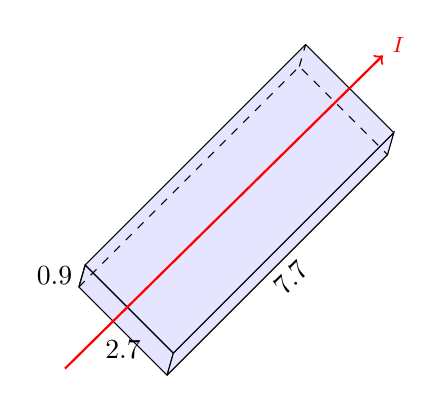
\begin{tikzpicture}[scale=2, x={(0.14cm,-0.14cm)},y={(0.04cm,0.14cm)},z={(-1.4cm,-1.4cm)}]
              \pgfmathsetmacro{\x}{4}
              \pgfmathsetmacro{\y}{1}
              \pgfmathsetmacro{\z}{1}
              \path (0,0,\y) coordinate (A) (\x,0,\y) coordinate (B) (\x,0,0) coordinate (C) (0,0,0)
              coordinate (D) (0,\z,\y) coordinate (E) (\x,\z,\y) coordinate (F) (\x,\z,0) coordinate (G)
              (0,\z,0) coordinate (H);
              \draw[fill=blue!10] (A)--(E)--(F)--(B);
              \draw[fill=blue!10] (A)-- node[below]{$2.7$} (B)-- node[below,sloped]{$7.7$} (C)--(G)--(F)--(B) (A)-- node[left]{$0.9$}(E)--(F)--(G)--(H)--(E);
              \draw [dashed,black] (A)--(D)--(C) (D)--(H);
              \draw[->, red, thick] (2, 1.3, 1.3)-- (2, 1, -0.15);
              \node[red] at (2, 1, -0.2) {\fontsize{8}{7} $I$};
          \end{tikzpicture}
      \end{center}
\end{minipage}

\item Parallel to $2.7$ (current goes through $0.9$, $7.7$ face): \\ 
\begin{minipage}{0.5\linewidth}
      \begin{center}
          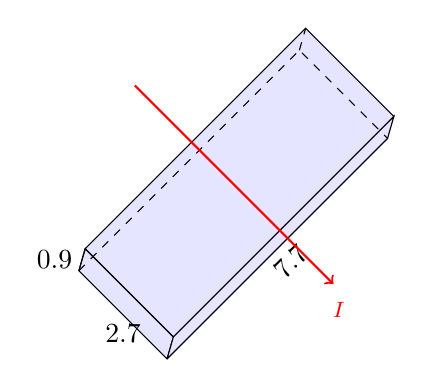
\begin{tikzpicture}[scale=2, x={(0.14cm,-0.14cm)},y={(0.04cm,0.14cm)},z={(-1.4cm,-1.4cm)}]
            \pgfmathsetmacro{\x}{4}
            \pgfmathsetmacro{\y}{1}
            \pgfmathsetmacro{\z}{1}
            \path (0,0,\y) coordinate (A) (\x,0,\y) coordinate (B) (\x,0,0) coordinate (C) (0,0,0)
            coordinate (D) (0,\z,\y) coordinate (E) (\x,\z,\y) coordinate (F) (\x,\z,0) coordinate (G)
            (0,\z,0) coordinate (H);
            \draw[fill=blue!10] (A)--(E)--(F)--(B);
            \draw[fill=blue!10] (A)-- node[below]{$2.7$} (B)-- node[below,sloped]{$7.7$} (C)--(G)--(F)--(B) (A)-- node[left]{$0.9$}(E)--(F)--(G)--(H)--(E);
            \draw [dashed,black] (A)--(D)--(C) (D)--(H);
            \draw[->, red, thick] (-1, 5.4, 0.8)-- (8, 5.4, 0.8);
            \node[red] at (8.3, 4.5, 0.8) {\fontsize{8}{7} $I$};
          \end{tikzpicture}
      \end{center}
\end{minipage}

\item Choices (i) and (iii) are tied for the maximum current flow.
\item The direction doesn't matter; the resistor is physically the same, so the current will be the same.
  \end{enumerate}
  
\end{multicols}

\meta {Emphasize/mention the different cross sectional area and length for each corresponding figure, and try to tie things back to Ohm’s law.
}

\ans{For a given supply voltage from a voltage source, the most current will flow when the resistance of the slab is smallest. We apply the geometrical resistance formula, $R=\frac{\rho_{Cu} L}{A}$. To maximize current, we need to minimize resistance, which requires minimizing $L$ and maximizing $A$. Two of the dimensions will comprise the area, and the third will form the length. Noticing that $0.9\si{\centi\meter}<2.7\si{\centi\meter}<7.7\si{\centi\meter}$, it follows that we want to feed current into the $2.7\si{\centi\meter}\times 7.7\si{\centi\meter}$ face and use $0.9\si{\centi\meter}$ as the length. Therefore, we select choice (i).
}


\itemSuppose we have $N$ wires similar to the one described in part (a). We align them side by side to form a bundle of wires. Find the overall resistance of this bundle. Are the wires connected in series or parallel? \\

    
    \ans{Since we have all $N$ wires aligned side by side, we are essentially expanding the cross-section area. This means that the new bundle will have a new cross-section area of $NA$, while its length remains the same ($L$). Hence, the overall resistance of the mega-wire will be:
    $$R_{mega} = \rho_{cu} \frac{L}{NA}$$
    This is similar to a parallel combination of $N$ wires. Note that the equivalent resistance is smaller for a parallel combination.
    }
    

\item\textbf{(PRACTICE)} Again how can we connect these $N$ identical wires so that the equivalent resistance is the highest?  \\
    
	\meta{In the next two questions, have students derive the equations for series and parallel resistors.}
    
    \ans{The key of this question is to start from the resistance equation:
    $$R = \rho\frac{l}{A}$$
    Algebraically, we want to maximize the value of $R$ for this question. Since $\rho$ is just a physical constant, we can't changes its value. Observing the fraction $\frac{l}{A}$, we can see that the overall length of the mega-wire should be as great as possible, while its cross section area should be kept as small as possible. How can we arrange $N$ wires in a way so that the overall new wire is as long as possible? \\
    We can arrange the wires in a single long line! This keeps the cross section area $A$ unchanged, but it has a length of $NL$. Applying the resistance equation, we have:
    $$R_{mega} = \rho_{cu}\frac{NL}{A}$$
    This configuration is exactly the same as a series connection of resistors. If you think in terms of the equivalent resistance for a series circuit, it also makes sense since we are summing up all the resistances.
    }
    
     \item\textbf{(PRACTICE)} Consider part (c) again, but this time, instead of $N$ copper wires, we split the number evenly between aluminum wires and copper wires. We arrange $N/2$ copper and $N/2$ aluminum wires side by side, and push them to form a new bundle of wires. What is the overall resistance of this wire? (In terms of $\rho_{cu}$, $\rho_{Al}$, $L$, and $A$) \\
    
    \ans{As we can see from part (c), when we are aligning the wires side by side, we are essentially arranging the wires to be parallel to each other. We can consider the bundle of wires to be a parallel combination of a bundle of copper wires and a bundle of aluminum wires! For both wires, they will have a length of $L$ and an overall cross section area of $(N/2)A$ (since we have $N/2$ wires for each category). Hence, applying the resistance equation again, we can find that:
    $$R_{Cu-bundle} = \rho_{Cu}\frac{L}{\frac{N}{2}A} = \rho_{cu}\frac{2L}{NA}$$
    $$R_{Al-bundle} = \rho_{Al}\frac{L}{\frac{N}{2}A} = \rho_{Al}\frac{2L}{NA}$$
    Now, since these 2 mega wires are parallel to each other, by equivalent resistance, we can find the overall resistance of the wire to be:
    $$R_{overall} = \frac{1}{\frac{1}{R_{Cu-bundle}} + \frac{1}{R_{Al-bundle}}} =\left( \frac{\rho_{Cu}\rho_{Al}}{\rho_{Cu} + \rho_{Al}} \right)\frac{2L}{NA}$$
 
}

\item\label{q:resistor:model} 
Now consider this \textit{core-shell nanowire} structure, where the outside shell made of Al and the inside made of Cu. $E_1$ and $E_2$ terminals are both connected to the faces of the Cu and Al structure, as shown in the picture. Draw a circuit diagram of the nanowire as a set of resistors, using $R_{\mathrm{Al}}$ for the resistance of the Al layer and $R_{\mathrm{Cu}}$ for the resistance of the Cu layer.




\begin{center}
\includegraphics[scale=1]{../q_resistor_model_figs/fig4.png}
\end{center}

\ans{

Given that we are contacting the full area and that current is flowing from end to end, each end can be treated as a node since each end will have the Au and Cu at the same potential. This means that we can model the core-shell nanowire as a set of parallel resistors.

%\begin{center}
%\includegraphics[scale = 0.3]{../q_resistor_model_figs/resistorcircuit.png}
%\end{center}

\begin{center}
\begin{circuitikz}
\draw (0, 0) to [short, o-] ++ (0, -1)
	to [short] ++ (-1, 0)
	to [R, l_=$R_{\mathrm{Au}}$] ++ (0, -3)
	to [short] ++ (1, 0)
	to [short, -o] ++ (0, -1);
\draw (0, -1) to [short] ++ (1, 0)
	to [R, l=$R_{\mathrm{Cu}}$] ++ (0, -3)
	to [short] ++ (-1, 0);
\end{circuitikz}
\end{center}

\vspace{-2in}

}

\vspace{2in}



\item Based on your model from part (f) and the parameters given below, find the equivalent resistance $R_{\mathrm{wire}}$ between $E_1$ and $E_2$.


\begin{center}
\begin{tabular}{ |c|c| } 
 \hline
 $\rho_{\mathrm{Al}}$ & $\SI{2e-8}{\ohm\meter}$ \\ 
 \hline
 $s_{\mathrm{Al}}$ & $\SI{10}{\nano\meter}$ \\ 
 \hline
 $\rho_{\mathrm{Cu}}$ & $\SI{1e-8}{\ohm\meter}$ \\ 
 \hline
 $s_{\mathrm{Cu}}$ & $\SI{5}{\nano\meter}$ \\ 
 \hline
 $l$ & $\SI{75}{\nano\meter}$ \\ 
 \hline
\end{tabular}
\end{center}

\ans{
Using the formula for resistance $R$, we can find the resistance of the Cu structure given the resistivity and the dimensions:
\[R = \rho \frac{l}{A} \implies R_{\mathrm{Cu}} = \rho_{\mathrm{Cu}} \frac{l}{s_{\mathrm{Cu}}^2} = \SI{1e-8}{\ohm\meter} \cdot \frac{\SI{75e-9}{\meter}}{\left(\SI{5e-9}{\meter}\right)^2} = \SI{30}{\ohm}\]

Using the formula for resistance $R$, we can find the resistance of the Al structure given the resistivity and the dimensions. In this case, the area of the Al structure is not just a square but rather the area of the Cu square subtracted from the area of the Al square (the area of a shell).

\[R_{\mathrm{Al}} = \rho_{\mathrm{Al}} \frac{l}{s_{\mathrm{Al}}^2 - s_{\mathrm{Cu}}^2} = \SI{2e-8}{\ohm\meter} \cdot \frac{\SI{75e-9}{\meter}}{\left(\SI{10e-9}{\meter}\right)^2 - \left(\SI{5e-9}{\meter}\right)^2} = \SI{20}{\ohm}\]

Because the two structures are in parallel, the total resistance $R_{\mathrm{wire}}$ is:
\[R_{\mathrm{wire}} = R_{\mathrm{Al}} \parallel R_{\mathrm{Cu}} = \frac{\SI{20}{\ohm} \cdot \SI{30}{\ohm}}{\SI{20}{\ohm} + \SI{30}{\ohm}} = \frac{\SI{600}{\ohm\squared}}{\SI{50}{\ohm}} = \SI{12}{\ohm}\]

}

%\vspace{5cm}

\end{enumerate}

